% =====================================================================
%  Bearings-only target localization: BEAR / DBEAR -- project report
%
%  Build (from this folder):   pdflatex report.tex   (run twice)
%  or:                         latexmk -pdf report.tex
%  All numbers, tables and figures are produced by make_figures.py.
% =====================================================================
\documentclass[11pt,a4paper]{article}

\usepackage[margin=2.4cm]{geometry}
\usepackage[T1]{fontenc}
\usepackage[utf8]{inputenc}
\usepackage{lmodern}
\usepackage{microtype}
\usepackage{amsmath,amssymb,amsthm}
\usepackage{bm}
\usepackage{graphicx}
\usepackage{booktabs}
\usepackage{array}
\usepackage{tabularx}
\usepackage[font=small,labelfont=bf]{caption}
\usepackage{subcaption}
\usepackage{xcolor}
\usepackage{algorithm}
\usepackage{algpseudocode}
\usepackage{enumitem}
\usepackage{listings}
\usepackage[section]{placeins}  % keep floats inside their section
\usepackage[hidelinks]{hyperref}
\usepackage[capitalise,noabbrev]{cleveref}

\graphicspath{{figures/}}
% Generated by report/make_figures.py -- do not edit by hand.
\newcommand{\angleBest}{335}
\newcommand{\angleBestPsi}{55}
\newcommand{\angleDip}{538}
\newcommand{\angleDipPsi}{8}
\newcommand{\angleNinety}{377}
\newcommand{\anglePeak}{2602}
\newcommand{\anglePeakPsi}{13}
\newcommand{\aspectAtEnd}{9}
\newcommand{\aspectEightHundred}{3.2}
\newcommand{\bfgsAgree}{7.5\times10^{-6}}
\newcommand{\bfgsItersTrue}{29.3}
\newcommand{\bfgsMs}{4.8}
\newcommand{\condFive}{8.4\times10^{5}}
\newcommand{\condNinety}{1100}
\newcommand{\condPeak}{2.0\times10^{5}}
\newcommand{\defaultSnr}{24.6}
\newcommand{\divProbMaxDev}{3.5}
\newcommand{\divProbRuns}{400}
\newcommand{\durLong}{317}
\newcommand{\durPeak}{3541}
\newcommand{\durPeakS}{40}
\newcommand{\durShort}{767}
\newcommand{\flagWrongBfgs}{0}
\newcommand{\flagWrongGn}{0}
\newcommand{\gnItersTrue}{5.4}
\newcommand{\gnMs}{0.5}
\newcommand{\hardCond}{2.8\times10^{5}}
\newcommand{\hardConvPct}{64.2}
\newcommand{\hardDivPct}{31.8}
\newcommand{\hardLowerPct}{100}
\newcommand{\hardMedNees}{37.4}
\newcommand{\hardPred}{36.2}
\newcommand{\hardRuns}{600}
\newcommand{\hardSnr}{0.35}
\newcommand{\initRuns}{100}
\newcommand{\initSuccessMin}{100}
\newcommand{\initTotal}{1100}
\newcommand{\locApps}{556}
\newcommand{\locCore}{2261}
\newcommand{\locGui}{2114}
\newcommand{\locTests}{1626}
\newcommand{\losMisalignEnd}{35}
\newcommand{\losMisalignMax}{5.8}
\newcommand{\majorMin}{361}
\newcommand{\majorMinT}{468}
\newcommand{\majorStart}{531}
\newcommand{\mcAvgHi}{4.125}
\newcommand{\mcAvgLo}{3.877}
\newcommand{\mcBiasMax}{0.064}
\newcommand{\mcCoverOne}{41.2}
\newcommand{\mcCoverThree}{98.9}
\newcommand{\mcCoverTwo}{86.2}
\newcommand{\mcFitMean}{55.74}
\newcommand{\mcFitOut}{4.9}
\newcommand{\mcFitVar}{107.8}
\newcommand{\mcItersMax}{7}
\newcommand{\mcItersMean}{5.3}
\newcommand{\mcKsFit}{0.01}
\newcommand{\mcKsNees}{0.29}
\newcommand{\mcMsPerRun}{0.4}
\newcommand{\mcNeesMean}{3.957}
\newcommand{\mcNeesOut}{5.3}
\newcommand{\mcNeesVar}{8.16}
\newcommand{\mcRuns}{2000}
\newcommand{\mcVarRatioMax}{1.08}
\newcommand{\mcVarRatioMin}{1.01}
\newcommand{\mcZtwoMax}{5.6}
\newcommand{\mcZtwoMin}{4.8}
\newcommand{\noiseConvMin}{100.0}
\newcommand{\noiseDivMax}{0.0}
\newcommand{\noiseMeanNeesSix}{7.3}
\newcommand{\noiseMedNeesSix}{2.9}
\newcommand{\noiseRatioOne}{0.97}
\newcommand{\noiseRatioSix}{1.33}
\newcommand{\noiseRuns}{400}
\newcommand{\nullResidual}{2.8\times10^{-19}}
\newcommand{\plainCondKm}{2500}
\newcommand{\plainCondM}{1.5\times10^{8}}
\newcommand{\rayDipDiv}{-0.00}
\newcommand{\rayDipOk}{-128.3}
\newcommand{\resCond}{1094}
\newcommand{\resFit}{44.20}
\newcommand{\resFitDof}{56}
\newcommand{\resFitHi}{78.57}
\newcommand{\resFitLo}{37.21}
\newcommand{\resIters}{5}
\newcommand{\resItersBfgs}{32}
\newcommand{\resNees}{0.690}
\newcommand{\resNeesTrue}{0.621}
\newcommand{\scaledCond}{1094}
\newcommand{\startBest}{400}
\newcommand{\startBestVal}{110}
\newcommand{\startBestZero}{240}
\newcommand{\startBestZeroVal}{511}
\newcommand{\startLateZeroVal}{798}
\newcommand{\startWorst}{80}
\newcommand{\startWorstVal}{811}
\newcommand{\testsTotal}{152}
\newcommand{\theoryCoverOne}{39.3}
\newcommand{\theoryCoverThree}{98.9}
\newcommand{\theoryCoverTwo}{86.5}
   % numerical results written by make_figures.py

% rows of a generated table (TeX primitive \input: safe inside tabular)
\makeatletter
\newcommand{\tablerows}[1]{\@@input generated/#1.tex }
\makeatother

% ------------------------------------------------------------------ notation
\newcommand{\R}{\mathbb{R}}
\newcommand{\x}{\bm{x}}
\newcommand{\xh}{\hat{\bm{x}}}
\newcommand{\xt}{\tilde{\bm{x}}}
\newcommand{\z}{\bm{z}}
\newcommand{\e}{\bm{e}}
\newcommand{\g}{\bm{g}}
\newcommand{\p}{\bm{p}}
\newcommand{\vv}{\bm{v}}
\newcommand{\dd}{\bm{d}}
\newcommand{\m}{\bm{m}}
\newcommand{\T}{^{\mathsf{T}}}
\newcommand{\J}{\bm{J}}
\newcommand{\Hm}{\bm{H}}
\newcommand{\Pm}{\bm{P}}
\newcommand{\Cm}{\bm{C}}
\newcommand{\Am}{\bm{A}}
\newcommand{\Id}{\bm{I}}
\newcommand{\Normal}{\mathcal{N}}
\newcommand{\E}{\mathbb{E}}
\DeclareMathOperator{\atantwo}{atan2}
\DeclareMathOperator{\wrap}{wrap}
\DeclareMathOperator{\diag}{diag}
\DeclareMathOperator{\rank}{rank}
\DeclareMathOperator{\tr}{tr}

\theoremstyle{plain}
\newtheorem{proposition}{Proposition}
\theoremstyle{remark}
\newtheorem*{remark}{Remark}

\lstset{basicstyle=\ttfamily\footnotesize, columns=fullflexible, frame=single,
        framerule=0.3pt, rulecolor=\color{black!30}, xleftmargin=4pt, xrightmargin=4pt}

\title{\textbf{Bearings-Only Target Localization}\\[4pt]
       \large Design, Theoretical Analysis and Experimental Verification\\
       of the BEAR and DBEAR Programs\\[6pt]
       \normalsize Short-term project report}
\author{\textit{[Author name]}}
\date{\today}

\begin{document}
\maketitle

\begin{abstract}
\noindent
A moving platform measures noisy bearings---directions only, never range---to
a target that moves with constant velocity. From these angles we must infer
the target's position and velocity, decide whether that is possible at all,
and quantify how well it can be done. This report documents the solution of
the project of Section~3.8.3 of Bar-Shalom, Li and Kirubarajan~\cite{bsl01}:
the program BEAR, which evaluates the Fisher information and the Cram\'er--Rao
lower bound (CRLB), computes the maximum likelihood estimate (MLE) and tests
it with the fitting error and the normalized estimation error squared (NEES),
and the program DBEAR, which draws the $g$-sigma position uncertainty
ellipses. Both are implemented in Python with command-line and graphical
interfaces and are covered by \testsTotal{} automated tests. The theoretical
analysis contributes a unit-invariant observability test, rank-aware
$\chi^2$ tests, and an analysis of \emph{range divergence}: for weak
maneuvers the likelihood can have no finite maximum, which a naive optimizer
reports as convergence. We derive the law
$P(\text{divergence}) \approx \Phi(-\rho_0/\sigma_{\rho_0})$ and confirm it by
simulation to within \divProbMaxDev{} percentage points. A Monte Carlo study
with \mcRuns{} runs confirms the efficiency and consistency of the estimator
(average NEES \mcNeesMean{} vs.\ 4; 2-sigma ellipse coverage
\mcCoverTwo\,\% vs.\ \theoryCoverTwo\,\%), and further experiments quantify the
effect of maneuver design, noise level and initialization. We close with the
lessons learned and directions for improvement.
\end{abstract}

\tableofcontents
\newpage

% =====================================================================
\section{Introduction}
\label{sec:intro}

Passive sensors such as sonar arrays, electronic support measures and
optical trackers observe the \emph{direction} to a target but not its
distance. Estimating the target's state from such bearings-only measurements
is the classical \emph{bearings-only target motion analysis}
problem~\cite{nardone84,aidala83}. It is hard for two reasons. First, the
measurement is a nonlinear function of the state. Second, and more
fundamentally, a single bearing contains no range information at all: range
can only be inferred from the way the bearings change while the observer
moves, and only if the observer's own motion is ``rich'' enough. A
constant-velocity target observed from a constant-velocity platform is
unobservable~\cite{nardone81}.

The project asks for two programs. \textbf{BEAR} accepts a scenario (true
target state, sampling, noise, platform motion and maneuvers, and an initial
estimate), evaluates the Fisher information matrix (FIM) and with it
observability and the CRLB, simulates noisy bearings, computes the MLE, and
evaluates the estimate statistically. \textbf{DBEAR} displays the
position-uncertainty ellipses. The algorithm that turns a $2\times2$
covariance matrix into a $g$-sigma ellipse must be documented.

\paragraph{Contributions.} Beyond a complete implementation of the
specification, the project produced:
\begin{enumerate}[nosep]
  \item a Python package with command-line and graphical versions of both
        programs, in-program help, a user guide, and \testsTotal{} automated
        tests (\cref{sec:solution});
  \item a unit-invariant numerical observability test and a proof of the
        rank deficiency of the non-maneuvering case (\cref{sec:observability});
  \item rank-aware fitting-error and NEES tests, with an argument for when
        NEES is not meaningful (\cref{sec:tests});
  \item an analysis of the non-existence of a finite MLE (range divergence),
        a detection rule, and the predictive law
        $P(\text{div})\approx\Phi(-\rho_0/\sigma_{\rho_0})$
        (\cref{sec:divergence});
  \item a reproducible experimental study of consistency, maneuver design,
        noise, divergence and optimization (\cref{sec:experiments}).
\end{enumerate}

\cref{sec:problem} states the problem, \cref{sec:theory} develops the
theory, \cref{sec:solution} describes the software, \cref{sec:experiments}
reports the experiments, \cref{sec:lessons} discusses lessons learned,
\cref{sec:improvements} lists ideas for improvement and \cref{sec:conclusion}
concludes.

% =====================================================================
\section{Problem statement}
\label{sec:problem}

\subsection{The assignment}

\cref{tab:spec} summarizes the specification. All inputs have defaults that
are read from the file \texttt{BEAR.DEF}.

\begin{table}[htbp]
\centering\small
\caption{Inputs and processing steps required of BEAR (Section~3.8.3 of~\cite{bsl01}).}
\label{tab:spec}
\begin{tabularx}{\linewidth}{@{}lX@{\hspace{1.5em}}lX@{}}
\toprule
\multicolumn{2}{@{}l}{\textbf{Inputs}} & \multicolumn{2}{l@{}}{\textbf{Processing}}\\
\midrule
A1 & true target parameter $\x$ at $t=0$       & B1 & FIM at the true $\x$; is it invertible (observability)?\\
A2 & sampling period $T$                         & B2 & inverse FIM (CRLB), if it exists\\
A3 & number of samples $n$                       & B3 & position covariance at every sampling time\\
A4 & noise variance $r$                          & B4 & noisy bearing measurements\\
A5 & platform initial position, velocity         & B5 & MLE by Newton--Raphson or quasi-Newton\\
A6 & platform maneuvers (velocities, $k_1$, $k_2$) & B6 & B1--B3 at the estimate\\
A7 & initial estimate for the minimization       & B7 & fitting error and its degrees of freedom\\
   &                                             & B8 & NEES and its probability limits\\
\bottomrule
\end{tabularx}
\end{table}

\subsection{Mathematical model}
\label{sec:model}

\paragraph{Target.} The target moves with constant velocity in the plane
$(\xi,\eta)$. Its parameter vector, defined at $t=0$, is
\begin{equation}
  \x = [\xi_0,\ \eta_0,\ \dot\xi,\ \dot\eta]\T, \qquad
  \p(t) = \Am(t)\,\x, \qquad
  \Am(t) = \begin{bmatrix}1&0&t&0\\0&1&0&t\end{bmatrix}.
  \label{eq:target}
\end{equation}

\paragraph{Platform.} The platform starts at $\p_p(0)$ with velocity
$\vv_0$. Maneuver leg $j$ imposes velocity $\vv_j$ for
$k_{1j}T \le t < k_{2j}T$. Outside every leg the platform moves with $\vv_0$,
and legs may not overlap. Integrating the piecewise-constant velocity gives
the closed form
\begin{equation}
  \p_p(t) = \p_p(0) + \vv_0 t + \m(t), \qquad
  \m(t) = \sum_j (\vv_j - \vv_0)\,
          \min\!\big(\max(t - k_{1j}T,\,0),\,(k_{2j}-k_{1j})T\big),
  \label{eq:platform}
\end{equation}
where $\m(t)$ is the displacement caused by the maneuvers.

\paragraph{Measurements.} Bearings are taken at $t_k = kT$, $k=1,\dots,n$.
With the relative position
$\dd_k = \p(t_k)-\p_p(t_k) = [\Delta\xi_k,\Delta\eta_k]\T$ and range
$\rho_k=\|\dd_k\|$,
\begin{equation}
  z_k = h_k(\x) + w_k, \qquad h_k(\x) = \atantwo(\Delta\eta_k, \Delta\xi_k),
  \qquad w_k \sim \Normal(0, r)\ \text{i.i.d.}
  \label{eq:meas}
\end{equation}
The bearing is measured counter-clockwise from the $\xi$ axis, in
$(-\pi,\pi]$. All angle differences are wrapped into $(-\pi,\pi]$ by
$\wrap(a)=\pi-\operatorname{mod}(\pi-a,2\pi)$.

\paragraph{Estimation problem.} Given $\z=[z_1,\dots,z_n]\T$, estimate $\x$,
decide whether $\x$ is identifiable, and quantify the uncertainty of
$\hat{\p}(t)=\Am(t)\xh$.

\paragraph{Assumptions where the specification is silent.}
The first measurement is at $t=T$, not at $t=0$. Outside the maneuver legs
the platform returns to its initial velocity. The same $r$ is used to
simulate the noise and inside the estimator.

\subsection{Reference scenario}

Unless stated otherwise, all experiments use the default scenario of
\cref{tab:scenario}. The platform sails north and turns east between
samples 20 and 40, then sails north again. The geometry is shown in
\cref{fig:geometry}.

\begin{table}[htbp]
\centering\small
\caption{Default scenario (\texttt{BEAR.DEF}); units m, s, rad.}
\label{tab:scenario}
\begin{tabular}{@{}lll@{}}
\toprule
Item & Value & Meaning\\
\midrule
A1 & $\x = [5000,\ 12000,\ -6,\ -2]\T$ & target 13\,km away, 6.3\,m/s\\
A2, A3 & $T=10$\,s, $n=60$ & 10-minute observation\\
A4 & $r=(1^\circ)^2 = 3.046\times10^{-4}$\,rad$^2$ & $\sigma = 1^\circ$\\
A5 & $\p_p(0)=[0,0]\T$, $\vv_0=[0,15]\T$ & north at 15\,m/s\\
A6 & $\vv_1=[15,0]\T$ for $k=20\ldots40$ & $90^\circ$ turn east for 200\,s\\
A7 & $\x^0=[2000,\ 8000,\ 0,\ 0]\T$ & rough initial guess\\
\bottomrule
\end{tabular}
\end{table}

% =====================================================================
\section{Theoretical analysis}
\label{sec:theory}

\subsection{Likelihood and Fisher information}

With Gaussian noise the log-likelihood is
$\ln\Lambda(\x) = -\tfrac{1}{2}\lambda(\x) + \text{const}$, where
\begin{equation}
  \lambda(\x) = \frac1r \sum_{k=1}^{n} \wrap\!\big(z_k-h_k(\x)\big)^2
  \label{eq:cost}
\end{equation}
is the normalized least-squares cost. Let $\bm{h}_x(k)=\partial h_k/\partial\x$
(a row vector). Since
$\partial\atantwo(\Delta\eta,\Delta\xi)/\partial\Delta\xi = -\Delta\eta/\rho^2$
and $\partial/\partial\Delta\eta = \Delta\xi/\rho^2$, \cref{eq:target} gives
\begin{equation}
  \bm{h}_x(k) = \frac{1}{\rho_k^2}\,
  \big[-\Delta\eta_k,\ \ \Delta\xi_k,\ \ -\Delta\eta_k t_k,\ \ \Delta\xi_k t_k\big].
  \label{eq:jacobian}
\end{equation}
The score is $\nabla\ln\Lambda = \frac1r\Hm\T(\z-\bm{h})$, where $\Hm$ stacks the
rows $\bm{h}_x(k)$. Its covariance is the FIM:
\begin{equation}
  \J(\x) = \E\big[\nabla\ln\Lambda\,\nabla\ln\Lambda\T\big]
         = \frac{1}{r}\sum_{k=1}^n \bm{h}_x(k)\T \bm{h}_x(k) = \frac1r \Hm\T\Hm .
  \label{eq:fim}
\end{equation}

\subsection{Cram\'er--Rao bound and position uncertainty}

If $\J$ is invertible, any unbiased estimator satisfies
$\operatorname{cov}(\xh)\succeq\Pm=\J^{-1}$~\cite{kay93}. The position at
time $t$ is the linear function $\p(t)=\Am(t)\x$, so its bound is
\begin{equation}
  \Cm(t) = \Am(t)\Pm\Am(t)\T =
  \begin{bmatrix}
    P_{11}+2tP_{13}+t^2P_{33} & P_{12}+t(P_{14}+P_{23})+t^2P_{34}\\
    \cdot & P_{22}+2tP_{24}+t^2P_{44}
  \end{bmatrix},
  \label{eq:poscov}
\end{equation}
which BEAR evaluates at every $t_k$ (step B3). DBEAR evaluates it at arbitrary
$t$, including extrapolation beyond $t_n$.

\subsection{Observability}
\label{sec:observability}

\begin{proposition}[Non-maneuvering platform]
\label{prop:null}
If the platform does not maneuver ($\m\equiv\bm0$), then
$\J\bm{n}_0=\bm{0}$ for
$\bm{n}_0 = \big[\p(0)-\p_p(0);\ \dot{\p}-\vv_0\big]$, so $\rank\J\le3$.
\end{proposition}
\begin{proof}
The relative position is $\dd(t) = (\p(0)-\p_p(0)) + (\dot\p-\vv_0)t$. The
parameter $\x(\alpha)=[\p_p(0)+\alpha(\p(0)-\p_p(0));\ \vv_0+\alpha(\dot\p-\vv_0)]$
has relative position $\alpha\dd(t)$ for every $\alpha>0$, and therefore the
same bearings. Hence $\partial h_k(\x(\alpha))/\partial\alpha = \bm{h}_x(k)\,\bm{n}_0=0$
at $\alpha=1$ for all $k$, so $\Hm\bm{n}_0=\bm0$ and $\J\bm{n}_0=\frac1r\Hm\T\Hm\bm{n}_0=\bm0$.
\end{proof}

Physically: a target at twice the range, whose velocity \emph{relative to the
platform} is also twice as large, produces identical bearings. A maneuver
adds $-\m(t)$ to $\dd(t)$, which does not scale with $\alpha$, and so breaks
the ambiguity. The singular values in \cref{tab:singular} show a numerically
exact null space ($\|\J\bm{n}_0\|/(\|\J\|\,\|\bm n_0\|)=\nullResidual$) without a
maneuver, and full rank with one.

\paragraph{A unit-invariant rank test.} The entries of $\J$ differ by many
orders of magnitude between position and velocity components, so
$\det\J$ and $\operatorname{cond}\J$ depend on the units. For the default
scenario, $\operatorname{cond}\J = \plainCondM$ in metres but $\plainCondKm$
in kilometres. BEAR therefore tests the diagonally scaled matrix
\begin{equation}
  \tilde\J = \bm{D}^{-1/2}\J\bm{D}^{-1/2}, \qquad \bm{D}=\diag(\J),
  \label{eq:scaled}
\end{equation}
and declares $\J$ singular if $\sigma_{\min}(\tilde\J)/\sigma_{\max}(\tilde\J)\le10^{-10}$.

\begin{proposition}[Unit invariance]
For any change of units $\x'=\bm{S}\x$ with $\bm{S}$ diagonal and positive,
$\tilde\J' = \tilde\J$.
\end{proposition}
\begin{proof}
$\J' = \bm{S}^{-1}\J\bm{S}^{-1}$ and $\bm{D}' = \bm{S}^{-2}\bm{D}$, so
$\tilde\J' = \bm{S}\bm{D}^{-1/2}\,\bm{S}^{-1}\J\bm{S}^{-1}\,\bm{D}^{-1/2}\bm{S}
= \bm{D}^{-1/2}\J\bm{D}^{-1/2}$, because diagonal matrices commute.
\end{proof}

The scaled condition number ($\scaledCond$ in both unit systems) is
therefore a meaningful, unit-free measure of observability.

\subsection{Maximum likelihood estimation}
\label{sec:mle}

The MLE minimizes $\lambda$ in \cref{eq:cost}. Its gradient and Hessian are
\begin{equation}
  \nabla\lambda = -\tfrac{2}{r}\Hm\T\e, \qquad
  \nabla^2\lambda = 2\J - \tfrac{2}{r}\sum_k e_k\nabla^2 h_k,
  \qquad \e = \wrap(\z-\bm h(\x)).
\end{equation}
At the true parameter, $\E[e_k]=0$, so the expected Hessian is $2\J$. Newton--Raphson
with the expected Hessian is \emph{Fisher scoring}, or Gauss--Newton, and
needs only first derivatives. BEAR uses Gauss--Newton with
Levenberg--Marquardt damping~\cite{levenberg44,marquardt63}
(\cref{alg:lm}). The damping is scaled by $\diag\bm A$, which makes the
iteration unit-invariant.

Convergence is tested with the \emph{Gauss--Newton decrement}
$\delta = \g\T\bm{A}^{+}\g$. Since
$\lambda(\x+\Delta\x)\approx\lambda(\x)-2\g\T\Delta\x+\Delta\x\T\bm A\Delta\x$,
$\delta$ is the cost reduction that an undamped step predicts. Because
$\lambda$ is dimensionless (it is on the $\chi^2$ scale), so is $\delta$, and
the tolerance $\delta\le10^{-10}$ needs no units.

The alternative is the quasi-Newton BFGS method~\cite{nocedal06}
(SciPy~\cite{scipy20}). It is run on rescaled coordinates
$\bm{y}=\sqrt{\diag\J(\x^0)}\odot(\x-\x^0)$ with the analytic gradient.

\begin{algorithm}[htbp]
\caption{Gauss--Newton with Levenberg--Marquardt damping (step B5).}
\label{alg:lm}
\begin{algorithmic}[1]
\Require bearings $\z$, initial estimate $\x^0$, tolerance $\tau$, divergence bound $R_{\max}$
\State $\x\gets\x^0$, \ $\mu\gets10^{-3}$
\For{$i=1,\dots,i_{\max}$}
  \State $\e\gets\wrap(\z-\bm h(\x))$; \ $\Hm\gets\partial\bm h/\partial\x$; \ $\bm A\gets\Hm\T\Hm/r$; \ $\g\gets\Hm\T\e/r$
  \If{$\g\T\bm A^{+}\g\le\tau$} \Return $\x$ \ (converged) \EndIf
  \Repeat
     \State solve $(\bm A+\mu\diag\bm A)\,\Delta\x=\g$
     \If{$\lambda(\x+\Delta\x)<\lambda(\x)$} \State $\x\gets\x+\Delta\x$, \ $\mu\gets\mu/10$, \ accept
     \Else \State $\mu\gets10\mu$ \EndIf
  \Until{accepted, or $\mu>10^{16}$ (stop: no descent possible)}
  \If{$\max_k\rho_k(\x)>R_{\max}$} \Return $\x$ \ (diverged, \cref{sec:divergence}) \EndIf
\EndFor
\end{algorithmic}
\end{algorithm}

\subsection{Statistical tests}
\label{sec:tests}

\begin{proposition}[Fitting error]
\label{prop:fit}
For the linearized model $\z = \Hm\x + \bm w$, the minimum cost satisfies
$\lambda(\xh)\sim\chi^2_{\,n-\rank\Hm}$.
\end{proposition}
\begin{proof}
The residual is $\e = (\Id-\Hm\Hm^{+})\bm w$, where $\Id-\Hm\Hm^+$ is an
orthogonal projector of rank $n-\rank\Hm$. Hence
$\e\T\e/r = (\bm w/\sqrt r)\T(\Id-\Hm\Hm^+)(\bm w/\sqrt r)$ is $\chi^2$ with
$n-\rank\Hm$ degrees of freedom.
\end{proof}

For the nonlinear model this holds asymptotically. BEAR uses
$n-\rank\J(\xh)$ degrees of freedom: $n-4$ normally, and $n-3$ without a
maneuver, where only three parameter combinations are fitted. Step B7
compares $\lambda(\xh)$ with the two-sided interval between the 2.5\,\%
and 97.5\,\% quantiles of $\chi^2_{n-4}$ (for 95\,\% confidence).

\paragraph{NEES.} If $\xt=\x-\xh\sim\Normal(\bm0,\J^{-1})$, then
$\epsilon=\xt\T\J\xt\sim\chi^2_4$, with 95\,\% interval $[0.484,\ 11.14]$
(step B8, with $\J$ evaluated at $\xh$). A single run says little. Over
$N$ independent runs $N\bar\epsilon\sim\chi^2_{4N}$, which gives a much
sharper Monte Carlo test.

When $\J(\xh)$ is singular the NEES is \emph{not meaningful}. The estimate lies
anywhere along the unobservable direction, and the null space of $\J(\xh)$ is
not that of $\J(\x)$ (it depends on $\xh$ through \cref{prop:null}). So
$\epsilon$ follows no $\chi^2$ law: in simulation its mean is about 5.7,
whereas $\chi^2_3$ would give 3. BEAR then reports the value without a
verdict.

\subsection{The \texorpdfstring{$g$}{g}-sigma ellipse}
\label{sec:ellipse}

Given a symmetric positive definite
$\Cm=\left[\begin{smallmatrix}C_{11}&C_{12}\\C_{12}&C_{22}\end{smallmatrix}\right]$,
DBEAR draws $\{\p:(\p-\hat\p)\T\Cm^{-1}(\p-\hat\p)=g^2\}$ as follows.
\begin{enumerate}[nosep]
\item \textbf{Eigenvalues.}
  $\lambda_1=\frac{C_{11}+C_{22}}{2}+\sqrt{\big(\frac{C_{11}-C_{22}}{2}\big)^2+C_{12}^2}$ and
  $\lambda_2=\det\Cm/\lambda_1$. Computing $\lambda_2$ from $\lambda_1\lambda_2=\det\Cm$
  avoids cancellation for the very thin ellipses typical of bearings-only
  problems.
\item \textbf{Orientation.} $\theta=\tfrac12\atantwo(2C_{12},\,C_{11}-C_{22})$.
\item \textbf{Semi-axes.} $a=g\sqrt{\lambda_1}$, $b=g\sqrt{\lambda_2}$.
\item \textbf{Points.} $\p(\varphi)=\hat\p+\bm R(\theta)[a\cos\varphi,\ b\sin\varphi]\T$, for
  $\varphi\in[0,2\pi]$.
\end{enumerate}

\begin{proposition}[Correctness and probability content]
Every point satisfies $(\p-\hat\p)\T\Cm^{-1}(\p-\hat\p)=g^2$. If
$\p\sim\Normal(\hat\p,\Cm)$, the ellipse contains $\p$ with probability
$1-e^{-g^2/2}$.
\end{proposition}
\begin{proof}
With $\Cm=\bm R\diag(\lambda_1,\lambda_2)\bm R\T$, where $\bm R=\bm R(\theta)$
(because $C_{11}-C_{22}=(\lambda_1-\lambda_2)\cos2\theta$ and
$2C_{12}=(\lambda_1-\lambda_2)\sin2\theta$), we get
$(\p-\hat\p)\T\Cm^{-1}(\p-\hat\p)=a^2\cos^2\!\varphi/\lambda_1+b^2\sin^2\!\varphi/\lambda_2=g^2$.
The quadratic form of a 2-D Gaussian is $\chi^2_2$, whose CDF is
$1-e^{-q/2}$; evaluating it at $q=g^2$ gives the probability.
\end{proof}

Thus $g=1,2,3$ contain $\theoryCoverOne$, $\theoryCoverTwo$ and
$\theoryCoverThree$\,\%, and $g=2.45$ contains 95\,\%. A 1-sigma ellipse
contains far less than the 68\,\% familiar from one dimension.

\subsection{Existence of the MLE: range divergence}
\label{sec:divergence}

\begin{proposition}[Limit at infinite range]
\label{prop:limit}
Let $\x(\alpha)$ scale the relative trajectory as in \cref{prop:null}, and let
$\beta_k^\infty=\atantwo$ of $(\p(0)-\p_p(0))+(\dot\p-\vv_0)t_k$ be the
bearings \emph{without} the maneuver parallax $\m$. Then
$\lambda(\x(\alpha))\to\lambda_\infty=\frac1r\sum_k\wrap(z_k-\beta^\infty_k)^2$
as $\alpha\to\infty$, and $\nabla\lambda\to\bm0$.
\end{proposition}
\begin{proof}
The relative position is $\alpha\big[(\p(0)-\p_p(0))+(\dot\p-\vv_0)t\big]-\m(t)$.
Its direction tends to that of the bracket as $\alpha\to\infty$, and
$\atantwo$ is continuous away from the origin. The gradient
\cref{eq:jacobian} scales as $1/\rho_k\to0$.
\end{proof}

Consequently, if the noisy data are fitted better by the parallax-free limit
than by every finite parameter, the infimum of $\lambda$ is \emph{not
attained}: no finite MLE exists. Every descent method then runs off to
infinite range, where the gradient vanishes, and a naive stopping test
reports convergence. This is a property of the data, not of the optimizer.

\paragraph{Predicting the divergence probability.}
Following the modified-polar-coordinate idea~\cite{aidala83}, parametrize the
target by the inverse initial range $\kappa=1/\rho_0$ and three
scale-invariant coordinates: the initial bearing $\beta_0$ and the relative
velocity per unit range, $\bm\nu=(\dot\p-\vv_0)/\rho_0$. Before the first
maneuver, the bearings do not depend on $\kappa$. Afterwards they are the
directions of $\bm u(\beta_0)+\bm\nu t-\kappa\,\m(t)$, which are smooth in
$\kappa$ \emph{through} $\kappa=0$, the point at infinity. In these
coordinates, divergence is simply the event that the unconstrained estimate
satisfies $\hat\kappa\le0$. If $\hat\kappa\approx\Normal(\kappa,\sigma_\kappa^2)$,
then, using $\sigma_\kappa/\kappa=\sigma_{\rho_0}/\rho_0$ (delta method),
\begin{equation}
  P(\text{divergence}) \approx \Phi\!\left(-\frac{\rho_0}{\sigma_{\rho_0}}\right),
  \label{eq:divlaw}
\end{equation}
where $\sigma_{\rho_0}$ is the CRLB standard deviation of the initial range.
The law tends to 50\,\% as observability vanishes, and it is negligible when
the range is well determined: for the default scenario
$\rho_0/\sigma_{\rho_0}=\defaultSnr$. \cref{sec:exp-divergence} confirms it
experimentally.

\paragraph{Detection.} BEAR stops and reports \emph{diverged} once
$\max_k\rho_k(\x)$ exceeds $10^3$ times the problem's length scale, which is
the larger of the initial-estimate range and the size of the platform track.

% =====================================================================
\section{Solution: software design}
\label{sec:solution}

\subsection{Architecture}

The computation is a pure-Python package, \texttt{bearloc}, built on
NumPy~\cite{numpy20}, SciPy~\cite{scipy20} and Matplotlib~\cite{hunter07}.
It is fully independent of the user interfaces (\cref{tab:modules}), so every
numerical step can be tested without a screen.

\begin{table}[htbp]
\centering\small
\caption{Software structure (lines include docstrings and comments).}
\label{tab:modules}
\begin{tabularx}{\linewidth}{@{}lXr@{}}
\toprule
Component & Content & Lines\\
\midrule
\texttt{bearloc} core & \texttt{model} (kinematics, bearings, Jacobian, FIM),
  \texttt{scenario} (A1--A7, \texttt{BEAR.DEF}), \texttt{estimation} (LM, BFGS,
  divergence), \texttt{stats} (rank test, $\chi^2$, NEES), \texttt{analysis}
  (B1--B8 pipeline, Monte Carlo), \texttt{ellipse}, \texttt{plotting},
  \texttt{report}, \texttt{samples} & \locCore\\
\texttt{bearloc.gui} & Tkinter windows for BEAR and DBEAR, ``?'' help icons and
  help browser, help texts & \locGui\\
programs & \texttt{bear.py}, \texttt{dbear.py} (command line);
  \texttt{bear\_gui.py}, \texttt{dbear\_gui.py} (windows); \texttt{build\_exe.py}
  (optional stand-alone \texttt{.exe}) & \locApps\\
\texttt{tests} & \testsTotal{} unit, statistical, theory and GUI tests & \locTests\\
\bottomrule
\end{tabularx}
\end{table}

\subsection{The programs}

\textbf{BEAR} (\cref{fig:screens}a) shows inputs A1--A7 on the left,
pre-filled from \texttt{BEAR.DEF} or from one of five sample scenarios.
Maneuver legs are edited in a small table. Pressing \emph{Run} (F5) executes
B1--B8 in a background thread. The Summary tab shows a colour-coded verdict for
observability, convergence, fitting error, NEES and an optional Monte Carlo
test, together with the estimate next to the truth and the geometry. Further
tabs hold the full numerical output. Every input and result carries a ``?''
icon: hovering shows a short explanation, and clicking opens a help browser
(\cref{fig:screens}c). Results are saved to \texttt{bear\_results.json}.

\textbf{DBEAR} (\cref{fig:screens}b) reads that file and draws the $g$-sigma
ellipses at user-chosen times (any $t\ge0$), with the covariance from B6 or
B3, optional bearing rays and zoom. A table lists each ellipse's centre,
semi-axes, orientation and whether it contains the truth.

The command-line versions offer the same functionality with interactive
prompts or a \texttt{--batch} mode. A build script packages the windows as
\texttt{BEAR.exe} and \texttt{DBEAR.exe}, as named in the assignment.

\begin{figure}[htbp]
\centering
\begin{subfigure}{\linewidth}\centering
  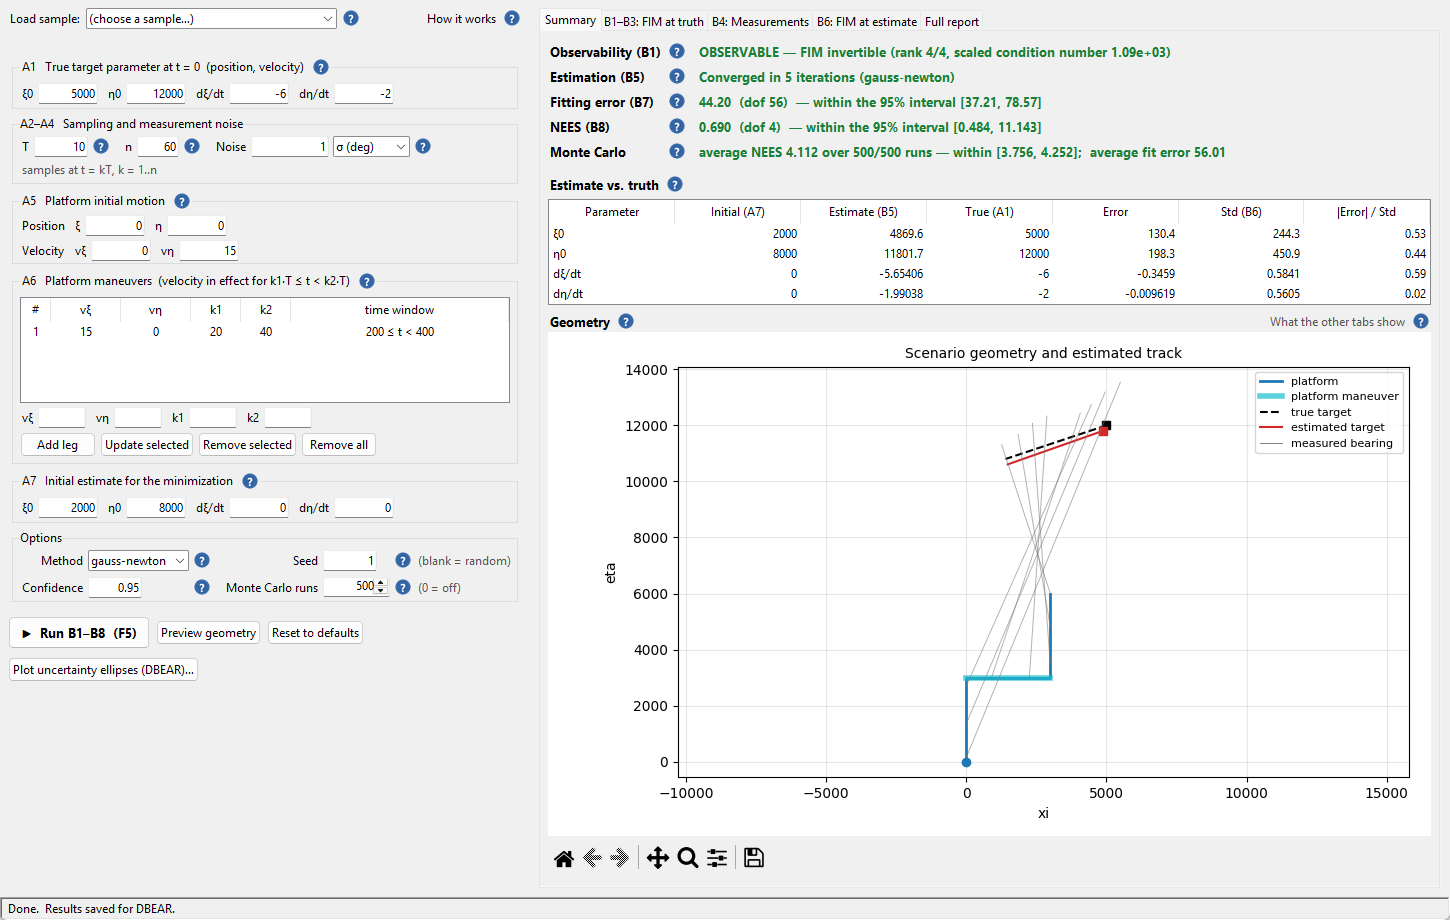
\includegraphics[width=0.92\linewidth]{screen_bear.png}
  \caption{BEAR after a run with 500 Monte Carlo runs.}
\end{subfigure}\\[4pt]
\begin{subfigure}{0.53\linewidth}\centering
  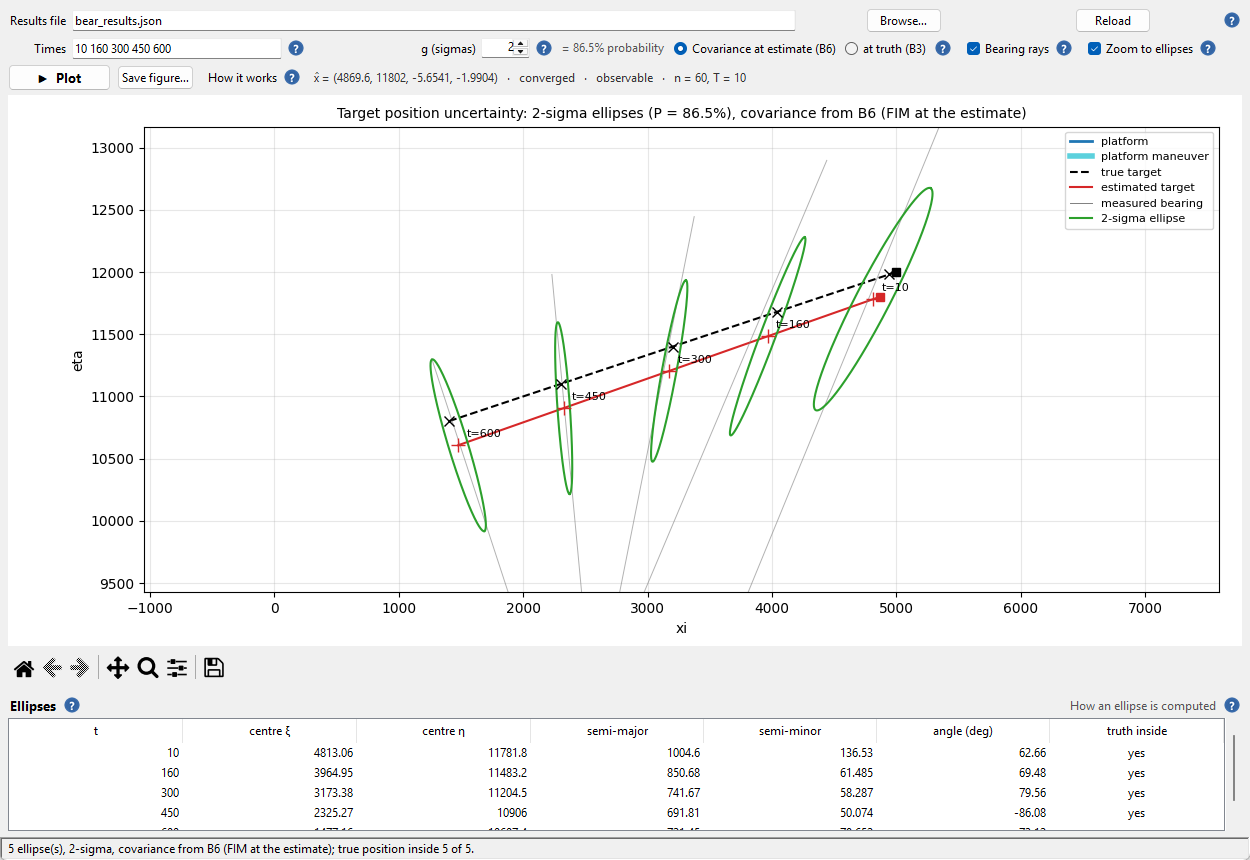
\includegraphics[width=\linewidth]{screen_dbear.png}
  \caption{DBEAR: 2-sigma ellipses and their table.}
\end{subfigure}\hfill
\begin{subfigure}{0.44\linewidth}\centering
  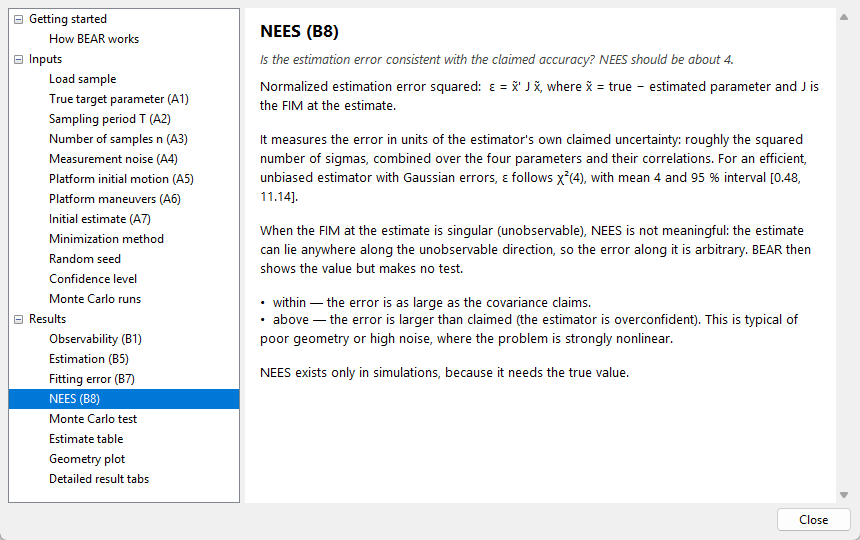
\includegraphics[width=\linewidth]{screen_help.png}
  \caption{Help browser opened from a ``?'' icon.}
\end{subfigure}
\caption{The graphical programs.}
\label{fig:screens}
\end{figure}

\subsection{Numerical safeguards}
\begin{itemize}[nosep]
\item Residuals are wrapped, so a target crossing the $\pm180^\circ$ bearing
      is handled correctly (tested).
\item The rank test and the LM damping are unit-invariant (\cref{sec:observability,sec:mle}).
\item $\J$, $\Pm$ and $\Cm$ are symmetrized; $\Pm$ is computed in scaled coordinates.
\item The ellipse's small eigenvalue is computed from the determinant (\cref{sec:ellipse}).
\item Range divergence is detected and reported as a failure (\cref{sec:divergence}).
\item When SciPy's BFGS stops with ``precision loss'', optimality is verified
      independently with the Gauss--Newton decrement (\cref{sec:exp-optim}).
\end{itemize}

\subsection{Verification strategy}

The \testsTotal{} tests (\cref{tab:tests}) run in about six seconds with the
standard library's \texttt{unittest}. They include analytic checks (Jacobian
against finite differences, the null vector of \cref{prop:null}, ellipse points
on the quadratic form), seeded statistical tests (the FIM equals the
covariance of the score, NEES $\sim\chi^2_4$, ellipse coverage, MLE variance
$\approx$ CRLB), end-to-end tests of all four programs, and GUI tests that
drive the hidden windows programmatically. All random numbers are seeded.

\begin{table}[htbp]
\centering\small
\caption{Automated tests per module.}
\label{tab:tests}
\begin{tabular}{@{}lr@{}}
\toprule
Test module & Tests\\
\midrule
\tablerows{tab_tests}
\midrule
Total & \testsTotal\\
\bottomrule
\end{tabular}
\end{table}

% =====================================================================
\section{Experimental results}
\label{sec:experiments}

All experiments are produced by \texttt{report/make\_figures.py}, which seeds
every random generator and writes every number quoted below. The complete set
runs in about 20 seconds; one estimate takes \gnMs\,ms with Gauss--Newton.

\subsection{A single run (steps B1--B8)}
\label{sec:exp-single}

For the default scenario, the FIM is invertible with scaled condition number
$\resCond$. The MLE converges in \resIters{} iterations from the rough initial
guess (\cref{tab:estimate}). Every error is below one standard deviation. The
fitting error $\resFit$ lies inside the 95\,\% interval
$[\resFitLo,\resFitHi]$ for $\chi^2_{\resFitDof}$, and the NEES $\resNees$ lies
inside $[0.484, 11.14]$. Using the FIM at the truth instead gives a NEES of
$\resNeesTrue$, almost the same, because $\J(\xh)\approx\J(\x)$ when the
estimate is accurate. \cref{fig:geometry} shows the geometry and the DBEAR
ellipses, and \cref{tab:ellipses} lists the ellipse parameters.

\begin{table}[htbp]
\centering\small
\caption{Single run of the default scenario (seed 1). Std (B6) is from
$\J(\xh)^{-1}$; CRLB is from $\J(\x)^{-1}$.}
\label{tab:estimate}
\begin{tabular}{@{}llrrrrrrr@{}}
\toprule
 & unit & initial & estimate & true & error & std (B6) & CRLB & $|$error$|$/std\\
\midrule
\tablerows{tab_estimate}
\bottomrule
\end{tabular}
\end{table}

\begin{figure}[htbp]
\centering
\begin{subfigure}{0.49\linewidth}\centering
  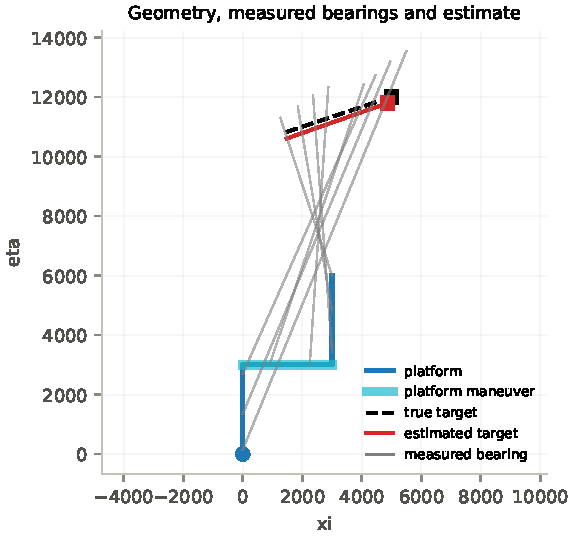
\includegraphics[width=\linewidth]{fig_geometry.pdf}
  \caption{Platform track with the maneuver (cyan), true and estimated target
  tracks, and eight measured bearings.}
\end{subfigure}\hfill
\begin{subfigure}{0.49\linewidth}\centering
  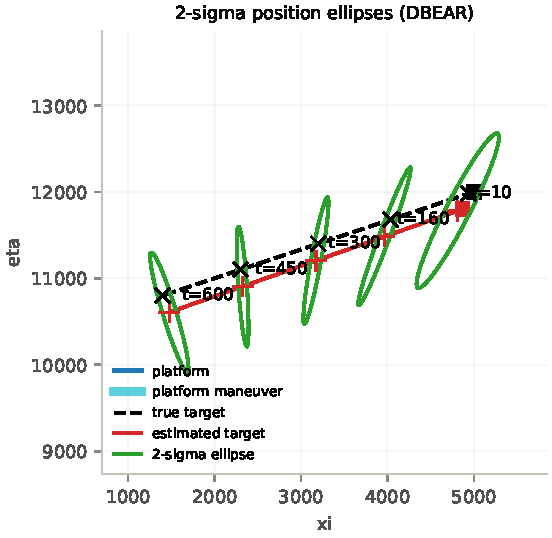
\includegraphics[width=\linewidth]{fig_ellipses.pdf}
  \caption{2-sigma ellipses at $t=10,160,300,450,600$\,s, centred at the
  estimate (+); the truth ($\times$) lies inside each one.}
\end{subfigure}
\caption{Default scenario: BEAR geometry and DBEAR uncertainty ellipses.}
\label{fig:geometry}
\end{figure}

\begin{table}[htbp]
\centering\small
\caption{2-sigma ellipses of \cref{fig:geometry}b (metres, degrees).}
\label{tab:ellipses}
\begin{tabular}{@{}rrrrrrc@{}}
\toprule
$t$ [s] & centre $\xi$ & centre $\eta$ & semi-major & semi-minor & angle & truth inside\\
\midrule
\tablerows{tab_ellipses}
\bottomrule
\end{tabular}
\end{table}

\subsection{Statistical consistency (Monte Carlo)}
\label{sec:exp-mc}

\Cref{tab:mc,tab:mcparams} and \cref{fig:consistency} summarize \mcRuns{}
independent runs of the default scenario. All runs converge, in
\mcItersMean{} iterations on average and at most \mcItersMax.

\begin{table}[htbp]
\centering\small
\caption{Monte Carlo study (\mcRuns{} runs) versus theory.}
\label{tab:mc}
\begin{tabular}{@{}lll@{}}
\toprule
Statement & Theory & Monte Carlo\\
\midrule
MLE unbiased & bias/std $=0$ & $|$bias$|$/std $\le\mcBiasMax$\\
MLE efficient & variance/CRLB $=1$ & $\mcVarRatioMin$ -- $\mcVarRatioMax$\\
Fitting error $\sim\chi^2_{56}$ & mean 56, variance 112 & $\mcFitMean$, $\mcFitVar$; KS $p=\mcKsFit$\\
\quad outside 95\,\% interval & 5\,\% & \mcFitOut\,\%\\
NEES $\sim\chi^2_4$ & mean 4, variance 8 & $\mcNeesMean$, $\mcNeesVar$; KS $p=\mcKsNees$\\
\quad outside $[0.484,11.14]$ & 5\,\% & \mcNeesOut\,\%\\
\quad average NEES in $[\mcAvgLo,\mcAvgHi]$ & yes & $\mcNeesMean$: yes\\
Ellipse coverage at $t=300$\,s, $g=1,2,3$ & $\theoryCoverOne$, $\theoryCoverTwo$, $\theoryCoverThree$\,\% & $\mcCoverOne$, $\mcCoverTwo$, $\mcCoverThree$\,\%\\
$|$error$|$/std $>2$, per component & 4.6\,\% & $\mcZtwoMin$ -- $\mcZtwoMax$\,\%\\
\bottomrule
\end{tabular}
\end{table}

\begin{table}[htbp]
\centering\small
\caption{Per-parameter Monte Carlo results.}
\label{tab:mcparams}
\begin{tabular}{@{}lrrrrr@{}}
\toprule
 & CRLB std & mean error & bias/std & error std & variance/CRLB\\
\midrule
\tablerows{tab_mc_params}
\bottomrule
\end{tabular}
\end{table}

\begin{figure}[htbp]
\centering
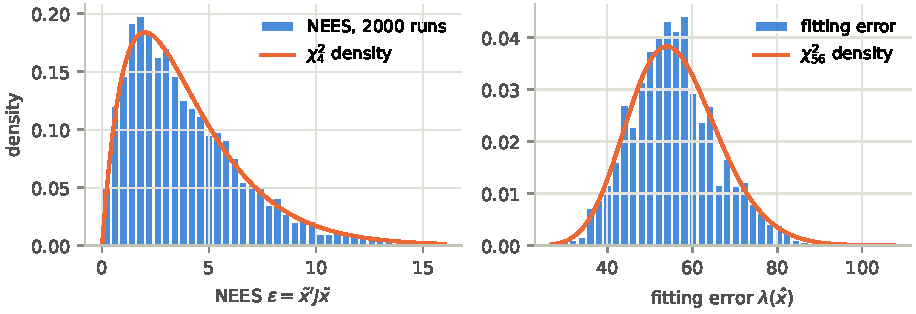
\includegraphics[width=\linewidth]{fig_consistency.pdf}
\caption{Distribution of NEES (left) and fitting error (right) over
\mcRuns{} runs, against the theoretical $\chi^2$ densities.}
\label{fig:consistency}
\end{figure}

The NEES distribution matches $\chi^2_4$ closely (Kolmogorov--Smirnov
$p=\mcKsNees$), and the ellipse coverage matches $1-e^{-g^2/2}$. The MLE is
efficient to within a few percent. The small residual bias (up to
$\mcBiasMax$ standard deviations, about three standard errors) and the
variance excess of up to $\mcVarRatioMax$ are expected: an MLE in a nonlinear
model is only \emph{asymptotically} unbiased and efficient. The mean and
variance of the fitting error are each within about one standard error of
theory, but the Kolmogorov--Smirnov test detects a slight shape difference
($p=\mcKsFit$). That is plausible: the $\chi^2$ law of \cref{prop:fit} is
exact only for linear models.

\subsection{Observability and uncertainty over time}
\label{sec:exp-observability}

\begin{table}[htbp]
\centering\small
\caption{Singular values of the scaled FIM $\tilde\J$ (\cref{eq:scaled}).}
\label{tab:singular}
\begin{tabular}{@{}lrrrrrr@{}}
\toprule
 & $\sigma_1$ & $\sigma_2$ & $\sigma_3$ & $\sigma_4$ & rank & condition\\
\midrule
\tablerows{tab_singular}
\bottomrule
\end{tabular}
\end{table}

\begin{figure}[htbp]
\centering
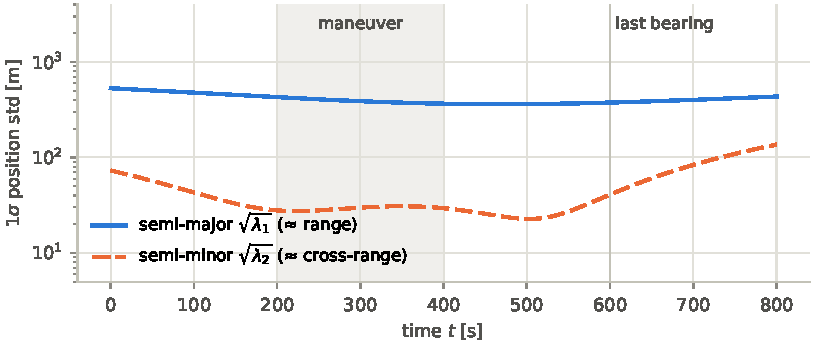
\includegraphics[width=\linewidth]{fig_crlb_time.pdf}
\caption{CRLB 1-sigma semi-axes of the position ellipse over time (default
scenario). The major axis is the range direction.}
\label{fig:crlbtime}
\end{figure}

\cref{fig:crlbtime} shows the bounds over time. The ellipse is elongated
throughout: its aspect ratio is about \aspectAtEnd{} at $t=600$\,s. Within the
observation window its major axis lies within $\losMisalignMax^\circ$ of the
line of sight, so bearings determine the direction well and the range
poorly. The range uncertainty shrinks from $\majorStart$\,m at $t=0$ to a
minimum of $\majorMin$\,m at $t=\majorMinT$\,s, shortly after the maneuver.
After the last bearing both axes grow, and the ellipse rotates away from the
line of sight ($\losMisalignEnd^\circ$ at 800\,s, aspect $\aspectEightHundred$)
as velocity uncertainty takes over.

\subsection{Maneuver design}
\label{sec:exp-maneuver}

\cref{fig:maneuver} varies the maneuver and reports the CRLB position
uncertainty $\sqrt{\tr\Cm(t)}$.

\begin{itemize}[nosep]
\item \textbf{Heading change (a).} The best turn is about
      $\angleBestPsi^\circ$ ($\angleBest$\,m, against $\angleNinety$\,m for
      $90^\circ$). Small turns behave non-monotonically: a dip of
      $\angleDip$\,m at $\angleDipPsi^\circ$, then a peak of $\anglePeak$\,m
      at $\anglePeakPsi^\circ$. Yet the scaled condition number decreases
      monotonically ($\condFive$ at $5^\circ$, $\condPeak$ at the peak,
      $\condNinety$ at $90^\circ$). For weak maneuvers, the poorly observed
      direction of $\J$ rotates with the turn angle, and at the peak it
      projects strongly onto the final position. A global observability
      measure therefore does not predict the uncertainty of a \emph{specific}
      quantity.
\item \textbf{Timing (b).} The best moment to turn depends on which time's
      position matters. For the position at $t_n$, a late turn is best
      (start $\startBest$\,s: $\startBestVal$\,m; start $\startWorst$\,s:
      $\startWorstVal$\,m). For the initial position, a turn starting around
      $\startBestZero$\,s is best ($\startBestZeroVal$\,m).
\item \textbf{Duration (c).} Longer turns help overall ($\durShort$\,m for
      10\,s, $\durLong$\,m for 400\,s), again with a non-monotone region
      for short turns (peak $\durPeak$\,m at $\durPeakS$\,s).
\end{itemize}

\begin{figure}[htbp]
\centering
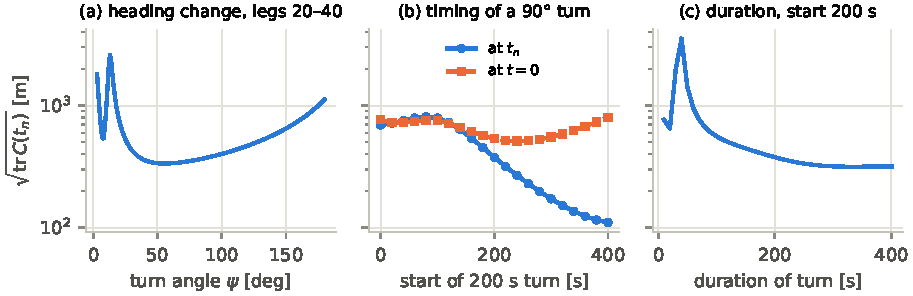
\includegraphics[width=\linewidth]{fig_maneuver.pdf}
\caption{CRLB position uncertainty versus (a) heading change of the leg
$k=20\ldots40$, (b) start of a 200\,s, $90^\circ$ turn, evaluated at $t_n$
and at $t=0$, and (c) duration of the turn.}
\label{fig:maneuver}
\end{figure}

\subsection{Noise level and the limits of the CRLB}
\label{sec:exp-noise}

\cref{tab:noise,fig:noise} repeat the default geometry with bearing noise
from $0.25^\circ$ to $6^\circ$ (\noiseRuns{} runs per level). The CRLB scales
exactly with $\sigma$. The MLE achieves it up to about $2^\circ$ (RMSE/CRLB
$\noiseRatioOne$ at $1^\circ$). Beyond that, efficiency degrades
($\noiseRatioSix$ at $6^\circ$) and the NEES acquires a heavy tail: the median
stays near the $\chi^2_4$ median ($\noiseMedNeesSix$ at $6^\circ$), while the
mean rises to $\noiseMeanNeesSix$. A minority of runs have errors far larger
than the inverse FIM claims. No run diverged at any noise level, which is
consistent with \cref{eq:divlaw}, since $\rho_0/\sigma_{\rho_0}\ge4$ here.

\begin{table}[htbp]
\centering\small
\caption{Effect of the noise level (default geometry, \noiseRuns{} runs per level).}
\label{tab:noise}
\begin{tabular}{@{}rrrrrrr@{}}
\toprule
$\sigma$ [deg] & CRLB at $t_n$ [m] & RMSE/CRLB & mean NEES & median NEES & converged [\%] & diverged [\%]\\
\midrule
\tablerows{tab_noise}
\bottomrule
\end{tabular}
\end{table}

\begin{figure}[htbp]
\centering
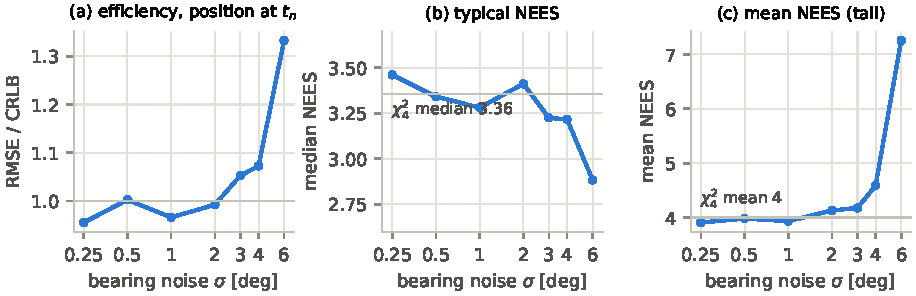
\includegraphics[width=\linewidth]{fig_noise.pdf}
\caption{Effect of the bearing noise: (a) efficiency, (b) median and (c)
mean NEES. Grey lines are the theoretical values.}
\label{fig:noise}
\end{figure}

\subsection{Range divergence}
\label{sec:exp-divergence}

The \emph{High noise, weak maneuver} sample (3$^\circ$, a small and short
turn, scaled condition number $\hardCond$) is only weakly observable. Out of
\hardRuns{} runs, \hardDivPct\,\% diverged, and in \hardLowerPct\,\% of these
the cost at the runaway estimate was \emph{lower} than at the true
parameter. This confirms that the likelihood itself has no finite maximum,
rather than the optimizer failing. Among the converged runs the median NEES
is $\hardMedNees$, so the CRLB badly understates the actual error.

\cref{fig:divergence} shows the cost along the ray of \cref{prop:limit},
relative to its limit $\lambda_\infty$. For a typical draw, $\lambda$ dips
well below $\lambda_\infty$ near the true range (minimum
$\lambda-\lambda_\infty=\rayDipOk$): a finite MLE exists. For a diverged draw, the curve approaches $\lambda_\infty$ from
above and never goes below it.

\cref{fig:divprob} tests the prediction \cref{eq:divlaw}. Two different
geometries---the hard sample with noise from $0.5^\circ$ to $6^\circ$, and the
default scenario with noise from $8^\circ$ to $24^\circ$---fall on the same
curve when plotted against $\rho_0/\sigma_{\rho_0}$. The largest deviation is
\divProbMaxDev{} percentage points (\cref{tab:divprob}). For the hard sample
at $3^\circ$ the law predicts $\hardPred$\,\% ($\rho_0/\sigma_{\rho_0}=\hardSnr$),
against $\hardDivPct$\,\% observed in the 600-run experiment above.
$\rho_0/\sigma_{\rho_0}$ is therefore the single number that predicts whether
the bearings-only MLE can fail.

\begin{figure}[htbp]
\centering
\begin{subfigure}{0.49\linewidth}\centering
  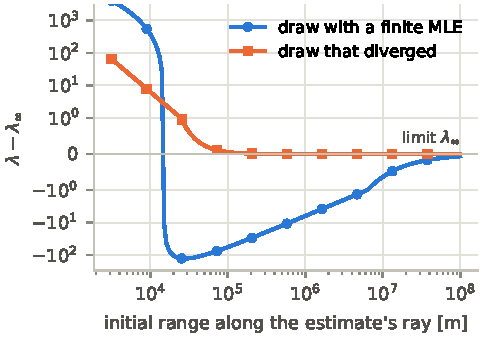
\includegraphics[width=\linewidth]{fig_divergence.pdf}
  \caption{$\lambda-\lambda_\infty$ along the estimate's ray (symmetric
  log scale).}
  \label{fig:divergence}
\end{subfigure}\hfill
\begin{subfigure}{0.49\linewidth}\centering
  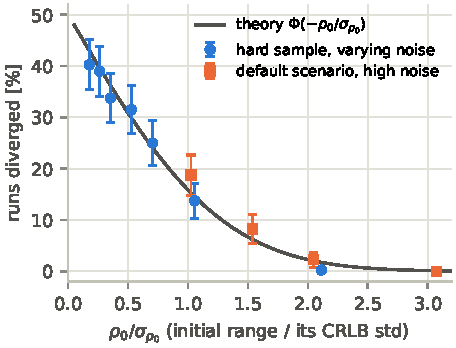
\includegraphics[width=\linewidth]{fig_divprob.pdf}
  \caption{Divergence probability: theory \cref{eq:divlaw} and Monte Carlo
  (\divProbRuns{} runs per point, $\pm2$ s.e.).}
  \label{fig:divprob}
\end{subfigure}
\caption{Range divergence: the likelihood without a finite maximum, and its prediction.}
\end{figure}

\begin{table}[htbp]
\centering\small
\caption{Predicted versus observed divergence probability.}
\label{tab:divprob}
\begin{tabular}{@{}lrrrr@{}}
\toprule
Geometry & $\sigma$ [deg] & $\rho_0/\sigma_{\rho_0}$ & predicted [\%] & observed [\%]\\
\midrule
\tablerows{tab_divprob}
\bottomrule
\end{tabular}
\end{table}

\subsection{Optimizers and initialization}
\label{sec:exp-optim}

\cref{fig:convergence} compares the two minimizers on the single run of
\cref{sec:exp-single}. Gauss--Newton converges in \resIters{}
iterations, almost quadratically. Strictly, it is quadratic only for
zero-residual problems, but here the residuals at the solution are small
compared with the curvature. BFGS needs \resItersBfgs. To test robustness, the
initial guess was placed on the first measured bearing at
$0.1$--$10$ times the true range, with zero velocity, for \initRuns{} noise
draws each (\cref{tab:init,fig:init}). Both methods found the global optimum
in \initSuccessMin\,\% of the \initTotal{} cases. Gauss--Newton needed
5--13 iterations and \gnMs\,ms; BFGS needed 27--52 iterations and
\bfgsMs\,ms. Their estimates agree to $\bfgsAgree$ standard deviations.

This experiment exposed a second false verdict. In about half of the runs
(49 of 100 in the first trial) SciPy's BFGS stopped with ``precision loss''
\emph{at} the optimum, so BEAR reported ``not converged'' for a correct
estimate. BEAR now verifies such terminations with the Gauss--Newton decrement
of \cref{sec:mle} (accepted if $\delta\le10^{-6}$). After the fix, the
convergence flag was wrong in \flagWrongBfgs{} of the \initTotal{} BFGS runs.

\begin{figure}[htbp]
\centering
\begin{subfigure}{0.49\linewidth}\centering
  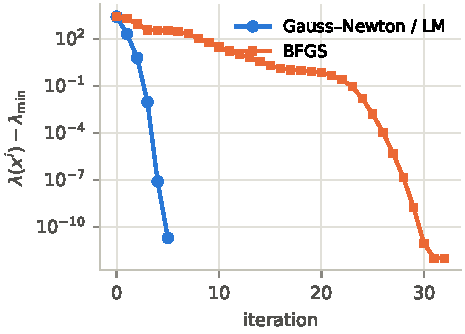
\includegraphics[width=\linewidth]{fig_convergence.pdf}
  \caption{Cost decrease per iteration (single run).}
  \label{fig:convergence}
\end{subfigure}\hfill
\begin{subfigure}{0.49\linewidth}\centering
  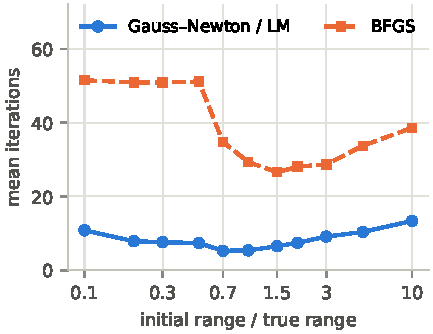
\includegraphics[width=\linewidth]{fig_init.pdf}
  \caption{Iterations versus initial-guess range (both methods reach the
  optimum in all cases).}
  \label{fig:init}
\end{subfigure}
\caption{Comparison of the minimizers.}
\end{figure}

\begin{table}[htbp]
\centering\small
\caption{Initial-guess robustness (\initRuns{} noise draws per row).}
\label{tab:init}
\begin{tabular}{@{}rrrrr@{}}
\toprule
initial / true range & GN found [\%] & GN iterations & BFGS found [\%] & BFGS iterations\\
\midrule
\tablerows{tab_init}
\bottomrule
\end{tabular}
\end{table}

\subsection{Sample scenarios}

\cref{tab:samples} summarizes the five sample scenarios shipped with the
programs (seed 1). They span the cases discussed above, from accurate and
consistent to unobservable and inconsistent.

\begin{table}[htbp]
\centering\small
\caption{The sample scenarios (seed 1). n/m: not meaningful (singular FIM).}
\label{tab:samples}
\begin{tabular}{@{}lllll@{}}
\toprule
Sample & scaled cond. & B5 & B7 fitting error & B8 NEES\\
\midrule
\tablerows{tab_samples}
\bottomrule
\end{tabular}
\end{table}

% =====================================================================
\section{Discussion and lessons learned}
\label{sec:lessons}

\subsection{Technical lessons}
\begin{enumerate}[leftmargin=*]
\item \textbf{``Converged'' is a claim that must be verified.} Two different
  mechanisms produced false verdicts: a likelihood without a finite maximum,
  where a vanishing gradient looks like convergence, and an optimizer library
  that reports failure at the optimum. Both were found only by checking the
  estimates against an independent criterion---the truth in simulation, and
  the Gauss--Newton decrement.
\item \textbf{Units are part of the mathematics.} A determinant or condition
  number test on $\J$ changes by orders of magnitude between metres and
  kilometres. Scale-invariant formulations (the scaled FIM, Marquardt
  damping, a dimensionless stopping criterion) remove arbitrary thresholds.
\item \textbf{A test statistic is only as good as its assumptions.} The
  degrees of freedom of the fitting error depend on $\rank\J$, and the NEES
  has no reference distribution when $\J$ is singular. Applying the textbook
  formulas blindly would produce confident but wrong verdicts.
\item \textbf{The CRLB is a local, high-SNR statement.} It is attained in the
  default scenario but fails gracefully, then abruptly, as observability
  weakens. The dimensionless ratio $\rho_0/\sigma_{\rho_0}$ captures this
  transition quantitatively.
\item \textbf{Geometry matters more than data volume.} Sampling the same
  window twice as densely shrinks the uncertainty only by $1/\sqrt2$, while
  the choice of maneuver changes it by an order of magnitude
  (\cref{fig:maneuver}). The ``best'' maneuver depends on which quantity
  matters.
\item \textbf{Single-run tests are weak.} One NEES value falls outside a
  95\,\% interval in 5\,\% of perfectly consistent runs; consistency can only
  be judged from many runs.
\end{enumerate}

\subsection{Process lessons}
\begin{enumerate}[leftmargin=*]
\item \textbf{Verify theory numerically and early.} Monte Carlo checks of
  every claimed property exposed the two false convergence verdicts, the
  wrong degrees of freedom, and several inaccurate statements in an early
  version of the documentation (for example, that a target ``twice as far
  and twice as fast'' gives the same bearings; the true ambiguity is in the
  \emph{relative} velocity).
\item \textbf{Separate computation from presentation.} Because the B1--B8
  pipeline knows nothing about the interfaces, the same tested code serves
  two command-line programs, two windows and the report generator.
\item \textbf{Make results reproducible by construction.} Seeded generators
  and numbers written directly into this report by \texttt{make\_figures.py}
  rule out transcription errors and make every figure regenerable.
\item \textbf{Record the assumptions.} The specification leaves several
  choices open (first sample time, velocity after a maneuver); stating them
  explicitly avoids silent disagreement with other implementations.
\item \textbf{Explain, do not only compute.} The in-program help and the
  user guide turned out to be as important as the algorithms for making the
  results interpretable, especially the warnings for unobservable or
  diverged cases.
\end{enumerate}

\subsection{Limitations}
The study is simulation-only, with Gaussian, i.i.d.\ bearing noise of known
variance and a non-maneuvering target. The covariance-based ellipses assume
local linearity, which \cref{sec:exp-noise,sec:exp-divergence} show to fail
for weak geometries. The divergence threshold factor $10^3$ is a heuristic.

% =====================================================================
\section{Ideas for improvement}
\label{sec:improvements}

\paragraph{Estimation.}
\begin{itemize}[nosep]
\item Estimate in \emph{modified polar coordinates}~\cite{aidala83} (inverse
  range). The model is smooth through infinite range, so a weakly observable
  case can be reported as ``range above $X$ with 95\,\% confidence'' instead
  of failing.
\item Add a weak prior on range (maximum a posteriori estimation), or a
  constraint, to regularize near-unobservable cases.
\item Use multiple starts along the first bearing, or a coarse grid in range,
  as a guard against local minima in harder geometries.
\item Estimate the noise variance from the fit
  ($\hat r = r\,\lambda(\xh)/(n-4)$) when $r$ is unknown.
\end{itemize}

\paragraph{Uncertainty quantification.}
\begin{itemize}[nosep]
\item Replace or complement the FIM ellipses by likelihood-ratio contours or
  profile-likelihood intervals in range. These capture the curved
  (``banana-shaped'') uncertainty of weak geometries.
\item Use the bootstrap or posterior sampling (MCMC, particle
  methods~\cite{ristic04}) when $\rho_0/\sigma_{\rho_0}$ is small.
\item Display $\rho_0/\sigma_{\rho_0}$ and the predicted divergence probability
  \cref{eq:divlaw} in BEAR as an at-a-glance reliability indicator.
\end{itemize}

\paragraph{Observer maneuver planning.} The experiments show that the
maneuver dominates performance. Optimizing it for a chosen criterion
(determinant or trace of $\J$, or the uncertainty at a time of interest), as
in~\cite{oshman99}, would be a natural extension: ``which turn should the
platform make?''

\paragraph{Models.} Maneuvering targets, three dimensions, unknown or
correlated noise, sensor biases, outliers (robust losses), multiple
platforms, and recursive filters (EKF, UKF, particle filters~\cite{ristic04})
for real-time tracking.

\paragraph{Software.} Packaging as an installable module, continuous
integration across platforms, vectorized Monte Carlo for speed, import of
recorded bearings from files (real data), and a code-signed installer for
the optional executables.

% =====================================================================
\section{Conclusion}
\label{sec:conclusion}

The project delivered complete BEAR and DBEAR programs for bearings-only
target localization, with command-line and graphical interfaces,
documentation and \testsTotal{} automated tests. The analysis established
the observability structure (rank deficiency without a maneuver, and a
unit-invariant test), the correct statistical tests (rank-aware degrees of
freedom, and when NEES is meaningful) and the $g$-sigma ellipse algorithm. It
also identified range divergence as a fundamental failure mode, together with
a law that predicts its probability from $\rho_0/\sigma_{\rho_0}$. The
experiments confirm the theory where it applies---the MLE is efficient and
consistent in the default scenario---and show quantitatively where and why it
stops applying. The most important lesson is methodological: in estimation
software, every claim (``converged'', ``consistent'', ``observable'') should
be checked against an independent criterion, and the most reliable way to do
that is a reproducible Monte Carlo study.

% =====================================================================
\begin{thebibliography}{99}\small

\bibitem{bsl01} Y.~Bar-Shalom, X.~R.~Li and T.~Kirubarajan,
  \emph{Estimation with Applications to Tracking and Navigation}.
  New York: Wiley, 2001.

\bibitem{nardone81} S.~C.~Nardone and V.~J.~Aidala,
  ``Observability criteria for bearings-only target motion analysis,''
  \emph{IEEE Trans.\ Aerospace and Electronic Systems}, vol.~AES-17, no.~2,
  pp.~162--166, 1981.

\bibitem{aidala83} V.~J.~Aidala and S.~E.~Hammel,
  ``Utilization of modified polar coordinates for bearings-only tracking,''
  \emph{IEEE Trans.\ Automatic Control}, vol.~AC-28, no.~3, pp.~283--294, 1983.

\bibitem{nardone84} S.~C.~Nardone, A.~G.~Lindgren and K.~F.~Gong,
  ``Fundamental properties and performance of conventional bearings-only
  target motion analysis,''
  \emph{IEEE Trans.\ Automatic Control}, vol.~AC-29, no.~9, pp.~775--787, 1984.

\bibitem{oshman99} Y.~Oshman and P.~Davidson,
  ``Optimization of observer trajectories for bearings-only target
  localization,''
  \emph{IEEE Trans.\ Aerospace and Electronic Systems}, vol.~35, no.~3,
  pp.~892--902, 1999.

\bibitem{kay93} S.~M.~Kay,
  \emph{Fundamentals of Statistical Signal Processing: Estimation Theory}.
  Englewood Cliffs, NJ: Prentice Hall, 1993.

\bibitem{levenberg44} K.~Levenberg,
  ``A method for the solution of certain non-linear problems in least
  squares,'' \emph{Quarterly of Applied Mathematics}, vol.~2, no.~2,
  pp.~164--168, 1944.

\bibitem{marquardt63} D.~W.~Marquardt,
  ``An algorithm for least-squares estimation of nonlinear parameters,''
  \emph{Journal of the SIAM}, vol.~11, no.~2, pp.~431--441, 1963.

\bibitem{nocedal06} J.~Nocedal and S.~J.~Wright,
  \emph{Numerical Optimization}, 2nd ed. New York: Springer, 2006.

\bibitem{ristic04} B.~Ristic, S.~Arulampalam and N.~Gordon,
  \emph{Beyond the Kalman Filter: Particle Filters for Tracking Applications}.
  Boston: Artech House, 2004.

\bibitem{numpy20} C.~R.~Harris \emph{et al.},
  ``Array programming with NumPy,'' \emph{Nature}, vol.~585, pp.~357--362, 2020.

\bibitem{scipy20} P.~Virtanen \emph{et al.},
  ``SciPy 1.0: fundamental algorithms for scientific computing in Python,''
  \emph{Nature Methods}, vol.~17, pp.~261--272, 2020.

\bibitem{hunter07} J.~D.~Hunter,
  ``Matplotlib: A 2D graphics environment,''
  \emph{Computing in Science \& Engineering}, vol.~9, no.~3, pp.~90--95, 2007.

\end{thebibliography}

% =====================================================================
\appendix
\section{Reproducing the results}
\label{app:repro}

From the project root:
\begin{lstlisting}
pip install -r requirements.txt
python -m unittest discover -s tests -t .     # all automated tests
python report/make_figures.py                 # figures, tables, numbers
python report/capture_screens.py              # program screenshots (needs a display)
cd report && pdflatex report.tex && pdflatex report.tex
\end{lstlisting}
The programs themselves are started with \texttt{python bear\_gui.py} and
\texttt{python dbear\_gui.py} (windows) or \texttt{python bear.py} and
\texttt{python dbear.py} (command line). \texttt{docs/user\_guide.md}
explains their use and \texttt{docs/algorithms.md} the mathematics.

\section{The defaults file}
\label{app:def}

\begin{lstlisting}
[target]
x_true = 5000, 12000, -6, -2      # A1: xi0, eta0, xi_dot, eta_dot
[sampling]
T = 10                            # A2
n = 60                            # A3
[noise]
r = 0.0003046174198               # A4: rad^2 (1 deg)
seed = 1
[platform]
position = 0, 0                   # A5
velocity = 0, 15
[maneuver 1]
velocity = 15, 0                  # A6: in effect for k1*T <= t < k2*T
k1 = 20
k2 = 40
[estimation]
x_init = 2000, 8000, 0, 0         # A7
method = gauss-newton
\end{lstlisting}

\end{document}
